% ******************************* Thesis Appendix A ****************************

\graphicspath{{Appendix1/Figs/}}

\chapter{Manual de usuario del emulador}

\section{Modo de uso}
Posicionándose en el directorio raíz, el emulador se inicia con el siguiente comando:
\begin{lstlisting}
sudo python start.py {RUTA_TOPOLOGIA}
\end{lstlisting}

El valor de \{RUTA\_TOPOLOGIA\} debe ser el path hacia el script Python que configura la topología. Para conocer los detalles de lo que debe hacer ese script, leer la sección A.2.

El script \textbf{start.py} realiza las siguientes funciones:
\begin{itemize}
	\item Carga la topología recibida por parámetro y la inicia.
	\item Borra el archivo utils/init\_json.json, en caso de que una ejecución previa lo haya creado. El propósito de este archivo se verá mas adelante.
	\item Llama al método \textbf{start} de cada nodo virtual. Cada una de las cuatro clases de nodos (RAUSwitch, RAUHost, RAUController y QuaggaRouter) tiene este método, que se encarga de inicializar y configurar el nodo.
\end{itemize}

Luego de iniciar, Mininet ofrece una línea de comandos con la que el usuario puede interactuar. Ejecutando el siguiente comando se puede obtener una terminal Linux en cualquiera de los nodos.
\begin{lstlisting}
xterm {NOMBRE_NODO}
\end{lstlisting}

De aquí en adelante en este manual de usuario, cuando se indique que hay que ejecutar un determinado comando en un nodo, se lo debe ejecutar en una consola xterm en dicho nodo.

Habiendo iniciado el entorno virtual, hay que llevar a cabo algunos pasos más para que sea totalmente funcional:
%%ATENCION!!
%https://github.com/santiagovidal/LiveCode/blob/master/ryu-master/ryu/app/proyecto/businessLogic/external_interfaces.py
\begin{enumerate}
	\item Esperar a que OSPF termine de distribuir las rutas y actualizar las bases de datos topológicas. Este proceso en general toma menos de un minuto, y varía de acuerdo al tamaño de la topología. Una manera de verificar esto es con el comando \textbf{route} y analizando la tabla de ruteo de los nodos.
	\item Ejecutar el comando \textbf{python telnetRouters.py} en cualquiera de los RAUSwitch. Este script escrito en Python se encarga de consultar la base de datos topológica de OSPF mediante Telnet, parsear la información y enviarla al controlador. Es importante asegurarse que el paso 1 esta completo antes de ejecutarlo, ya que en caso contrario la base de datos de OSPF estará incompleta y se estarán enviando datos incorrectos. Luego de recibir la topología, el controlador todavía necesita la siguiente información de cada RAUSwitch: nombres de interfaces, direcciones IP y direcciones MAC. Para obtener esta información, se conecta automáticamente con el nodo que tiene levantado el Web Service que hace disponible la información de cada nodo. El nodo que levanta el Web Service es el controlador mismo (es decir, se conecta consigo mismo mediante localhost) pero puede ser cualquiera, siempre y cuando esté ejecutando el script \textbf{utils/wsOVS.py}. Este script es el sustituto que se creó para suplantar a \textbf{wsSNMP.py} (recordar sección 3.3.5).
	\item Para poder crear servicios en RAUFlow, se debe indicar cuales RAUSwitch son de borde y cuales no. En el caso de los que son de borde, también se debe especificar la dirección IP y MAC del nodo CE (que típicamente será un RAUHost o QuaggaRouter) con el que el RAUSwitch está conectado. Tradicionalmente esto se hace en la interfaz web de RAUFlow, pero esto resulta tedioso y lento si se tienen muchos nodos. Para acelerar este proceso se creó un script llamado \textbf{nodeInits.py} que se puede ejecutar desde cualquier nodo, y se encarga de enviar toda esa información al controlador mediante pedidos HTTP. La ejecución de este script es opcional; si el usuario desea puede ingresar los datos mediante la interfaz web. El script envía los datos que se encuentren en el archivo \textbf{init\_json.json}, y dicho archivo es creado automáticamente cuando se levanta el emulador. En caso de hacerse, la ejecución de este script debe ser posterior a la de telnetRouters.py, ya que en caso contrario se estarían mandando datos de nodos que el controlador todavía no conoce. En la sección A.2 se explicará como indicarle al emulador que nodos son de borde, así como las direcciones de los nodos CE.
\end{enumerate}

Luego de que el entorno está levantado y listo para usarse, se puede empezar a crear servicios. Para usar la interfaz web de RAUFlow se debe levantar un explorador desde el nodo controlador. Esto se puede lograr primero iniciando una consola xterm en dicho nodo, y luego ejecutando el comando que inicie el explorador. Una vez en la interfaz web de RAUFlow, se puede interactuar con ella de forma normal.

\section{Cómo interactuar con cada instancia de Open vSwitch}
Como se explica en el capítulo 3, cada RAUSwitch tiene su propia instancia de Open vSwitch ejecutándose en modo userspace. Esto modifica un poco la manera de usar sus comandos, ya que cada comando se debe 'apuntar' a la instancia con la que se desea interactuar.

Cada RAUSwitch tiene un directorio bajo /tmp donde se almacenan los archivos relacionados con su instancia de Open vSwitch y Quagga. El siguiente diagrama explica la estructura de archivos correspondiente a un nodo llamado 'switch1'. 
\dirtree{%
	.1 /.
	.2 tmp.
	.3 switch1.
	.4 ovs.
	.5 db.sock.
	.5 ovs-vswitchd.ctl.
	.4 quagga.
}

El diagrama muestra dos archivos que son vitales para poder comunicarse con la instancia de Open vSwitch del nodo 'switch1'. Estos son: \textbf{db.sock} y \textbf{ovs-vswitchd.ctl}. El propósito de estos archivos se explicará más adelante. Los demás archivos que se mantienen en estos directorios son los relacionados con Quagga, y se omiten por simplicidad.

Open vSwitch tiene varias herramientas que permiten consultar datos y realizar configuraciones. Las de interés en este contexto son: ovs-appctl, ovs-vsctl, ovs-ofctl y ovs-dpctl. A continuación se explicará en que consiste cada una y como usarla apuntando a un nodo específico.
\begin{itemize}
	\item \textbf{ovs-appctl} \cite{ovs-appctl} es una herramienta que permite enviarle comandos al demonio ovs-vswitchd. Se le puede consultar cosas como flujos, logs, etc, así como realizar configuraciones en tiempo de ejecución. El entorno virtual tendrá múltiples instancias de este demonio ejecutando, así que es necesario indicar a qué instancia debe ser dirigido un comando. Esto se hace con la opción \textbf{-t} o \textbf{--target} seguido por el socket de Unix en el cual la instancia está escuchando por conexiones de control. Aquí entra en juego el archivo \textbf{ovs-vswitchd.ctl} mencionado anteriormente. Al iniciarse, cada instancia de Open vSwitch almacenará ese socket en el directorio privado de su nodo. Por lo tanto, para apuntar un comando 'ovs-appctl' hacia un nodo específico se debe hacer: \textit{ovs-appctl --target=/tmp/nombre\_nodo/ovs/ovs-vswitchd.ctl nombre\_comando}.
	\item \textbf{ovs-vsctl} \cite{ovs-vsctl} permite conectarse con el proceso ovsdb-server, quien se encarga de mantener la base de datos de configuración de Open vSwitch. ovs-vsctl permite consultar y modificar dicha base de datos. Igual que en el caso de ovs-appctl, se debe especificar a que instancia se desea apuntar el comando. Esto se logra con la opción \textbf{--db}, que indica el modo de conexión que se utilizará. Este puede ser: un socket de Unix o la red. En caso de usar un socket de Unix, se debe indicar la ruta al archivo \textbf{db.sock} que le corresponde al nodo, de la siguiente manera: \textit{ovs-vsctl --db=unix:/tmp/nombre\_nodo/ovs/db.sock nombre\_comando}. Por otro lado, si se desea enviar el comando a través de la red, se debe ejecutar: \textit{ovs-vsctl --db=tcp:dirección\_ip:6640 nombre\_comando} usando la dirección IP del nodo de interés.
	\item \textbf{ovs-ofctl} \cite{ovs-ofctl} permite monitorear y administrar el switch OpenFlow. Por ejemplo, un uso frecuente es el de consultar el contenido de las tablas de flujos de un switch, que se hace con el siguiente comando: \textit{ovs-ofctl -O OpenFlow13 dump-flows nombre\_nodo}. A diferencia de las herramientas anteriores, no hace falta indicar de una forma especial a qué nodo apunta el comando. Alcanza con ejecutarlo en una consola xterm en el nodo que se busca administrar.
	\item \textbf{ovs-dpctl} \cite{ovs-dpctl} es un programa que permite consultar y administrar los flujos de los datapaths externos a ovs-vswitchd, como el datapath del kernel. El datapath del kernel no es utilizado en el entorno (debido a las múltiples instancias de Open vSwitch), por lo tanto no es posible usar esta herramienta. Para administrar el datapath en el userspace (también llamado netdev) se puede utilizar la familia de comandos \textit{dpctl/*} de ovs-appctl. Por ejemplo, \textit{ovs-appctl  --target=/tmp/nombre\_nodo/ovs/ovs-vswitchd.ctl dpctl/show} muestra las estadísticas del cache de flujos para un determinado nodo.
\end{itemize}

\section{API para configurar las topologias}
La API que se debe usar para crear y personalizar las topologias es, en esencia, la misma que Mininet estándar. Cada topología debe ser configurada por un script Python, que debe definir una subclase de la clase \textit{Topo} de Mininet. A dicha subclase se le debe agregar nodos y enlaces mediante los métodos \textit{addHost}, \textit{addSwitch}, y \textit{addLink}. En el caso de los dos primeros, es necesario indicar la clase de nodo que se está agregando, y los parámetros necesarios para inicializar esa clase. Como se explica en el capítulo 3, se crearon cuatro nuevas clases de nodos, y a continuación se detallan los parámetros que se pueden usar en sus constructores. Los resaltados con * son obligatorios. \\

\underline{RAUSwitch}
\begin{itemize}
	\item \textbf{nombre} \textcolor{red}{*}. Nombre del switch.
	\item \textbf{ips} \textcolor{red}{*}. Lista con todas las direcciones IP (en formato CIDR, A.B.C.D/E) para el switch.
	\item \textbf{dpid} \textcolor{red}{*}. Datapath ID del switch. Debe ser un string hexadecimal de largo 16. En caso de no proveer este valor, el datapath ID se derivará del nombre del switch. Por ejemplo: si el nombre es \textit{switch8}, su datapath ID será 8.
	\item \textbf{controller\_ip} \textcolor{red}{*}. Dirección IP del controlador.
	\item \textbf{border}. Número entre 0 o 1 que indica si el switch es de borde o no. Si no se provee, se asume que border=0.
	\item \textbf{ce\_ip\_address}. Dirección IP del nodo CE con el que está conectado. Solo aplica si el switch es de borde.
	\item \textbf{ce\_mac\_address}. Dirección MAC del nodo CE con el que está conectado. Solo aplica si el switch es de borde.
\end{itemize}

\underline{RAUHost}

\begin{itemize}
	\item \textbf{nombre} \textcolor{red}{*}. Nombre del host.
	\item \textbf{ips} \textcolor{red}{*}. Lista con todas las direcciones IP (en formato CIDR, A.B.C.D/E) para el host. En general tendrá una única dirección IP, pero por las dudas se permite que tenga varias.
	\item \textbf{gw}.  Dirección IP del default gateway.
	\item \textbf{ce\_mac\_address}. En caso de que el host se esté usando como nodo CE, este parámetro indica la dirección MAC que debe tener la interfaz que lo conecta con el RAUSwitch. En caso de existir, dicha interfaz debe ser la menor de todas.
\end{itemize}

\underline{RAUController}

\begin{itemize}
	\item \textbf{nombre} \textcolor{red}{*}. Nombre del controlador.
	\item \textbf{ips} \textcolor{red}{*}. Lista con todas las direcciones IP (en formato CIDR, A.B.C.D/E) para el controlador. En general tendrá una única dirección IP, pero por las dudas se permite que tenga varias.
\end{itemize}

\underline{QuaggaRouter}

\begin{itemize}
	\item \textbf{nombre} \textcolor{red}{*}. Nombre del router.
	\item \textbf{ips} \textcolor{red}{*}. Lista con todas las direcciones IP (en formato CIDR, A.B.C.D/E) para el router.
	\item \textbf{gw}.  Dirección IP del default gateway.
	\item \textbf{ce\_mac\_address}. En caso de que el router se esté usando como nodo CE, este parámetro indica la dirección MAC que debe tener la interfaz que lo conecta con el RAUSwitch. En caso de existir, dicha interfaz debe ser la menor de todas.
\end{itemize}

Cada nodo tendrá un conjunto de interfaces de red, definidas de acuerdo a como se creen los enlaces de ese nodo. Por ejemplo, el siguiente fragmento de código crea enlaces entre tres nodos llamados \textit{switch1}, \textit{switch2} y \textit{switch3}:
\begin{lstlisting}
addLink(switch1, switch2, 0, 0)
addLink(switch1, switch3, 1, 0)
\end{lstlisting}

Los últimos dos parámetros indican qué número de interfaz debe tener cada nodo. La primera línea significa que tanto el switch1 como el switch2 tendrán eth0 conectadas a ese enlace. La segunda indica que el switch1 usará eth1 para el enlace, mientras que el switch3 usará eth0. Es importante prestar especial atención a esto, ya que el parámetro \textit{ips} con el que se inicializa cada nodo debe cumplir ciertas reglas:
\begin{itemize}
	\item La cantidad de direcciones IP debe coincidir con la cantidad de interfaces de red.
	\item Las direcciones IP serán asignadas según el orden en el que están en la lista, empezando desde la interfaz más baja.
	\item Si se trata de un RAUSwitch, la primera interfaz (y por ende la primera dirección IP de la lista) debe ser la de la red de gestión.
	\item Si se trata de un RAUSwitch y es de borde, la última interfaz debe ser la que lo conecte con el nodo CE, ya sea un RAUHost o un QuaggaRouter.
	\item Si se trata de un RAUHost o QuaggaRouter que actúa como nodo CE (es decir, está conectado a un RAUSwitch), la primera interfaz debe ser la que lo conecte con el RAUSwitch.
\end{itemize}

\subsection{Ejemplo}
\begin{figure}[t]
	\caption{Topología de ejemplo}
	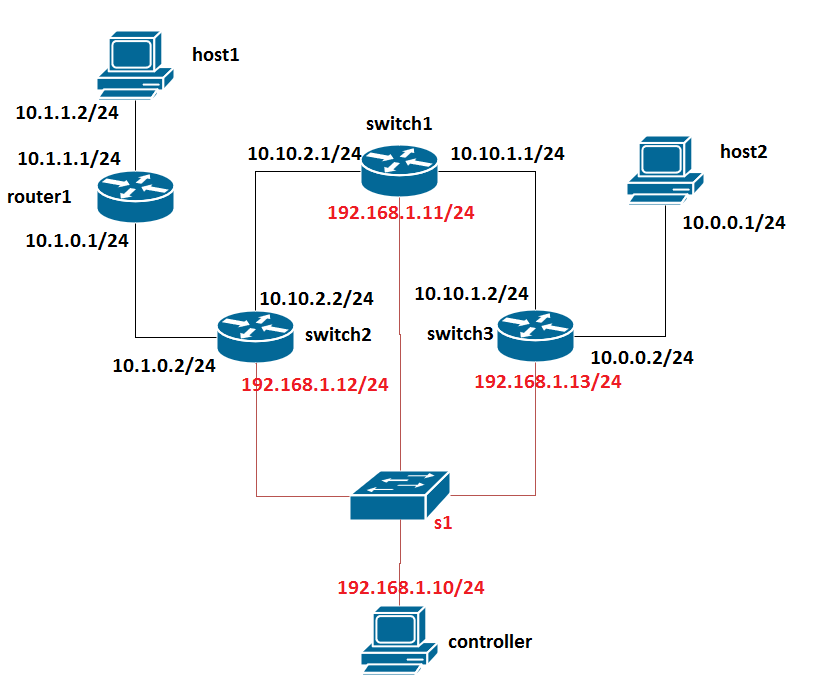
\includegraphics[width=\textwidth,height=\textheight,keepaspectratio]{topo-ejemplo}
	\centering
	\label{fig:topo_ejemplo}
\end{figure}

En la figura \ref{fig:topo_ejemplo} se puede ver una pequeña topología de ejemplo que consiste de 3 RAUSwitch, 1 QuaggaRouter actuando como CE, un RAUHost actuando como CE y otro RAUHost conectado al QuaggaRouter. También se puede ver la red de gestión marcada con rojo. A continuación se muestra el código que implementa esa topología:

\begin{minted}{python}
from mininet.topo import Topo
from rau_nodes import RAUSwitch, QuaggaRouter, RAUController, RAUHost

class CustomTopology( Topo ):
  def __init__( self ):
	Topo.__init__( self )

	# Hosts
	host1 = self.addHost('host1',
		ips=['10.1.1.2/24'],
		cls=RAUHost)
	host2 = self.addHost('host2',
		ips=['10.0.0.1/24'],
		ce_mac_address='00:00:00:00:00:02',
		cls=RAUHost)
	
	# Router	
	router1 = self.addHost('router1',
		ips=['10.1.0.1/24', '10.1.1.1/24'],
		ce_mac_address='00:00:00:00:00:01',
		cls=QuaggaRouter)
		
	# Switches
	# Los dpid se omiten ya que se pueden derivar de los nombres
	switch1 = self.addHost('switch1',
		ips=['192.168.1.11/24','10.10.2.1/24','10.10.1.1/24'],
		controller_ip="192.168.1.10",
		cls=RAUSwitch)

	switch2 = self.addHost('switch2',
		ips=['192.168.1.12/24','10.10.2.2/24','10.1.0.2/24'],
		controller_ip="192.168.1.10",
		border=1, ce_ip_address='10.1.0.1',
		ce_mac_address='00:00:00:00:00:01',
		cls=RAUSwitch)
		
	switch3 = self.addHost('switch3',
		ips=['192.168.1.13/24','10.10.1.2/24','10.0.0.2/24'],
		controller_ip="192.168.1.10",
		border=1, ce_ip_address='10.0.0.1',
		ce_mac_address='00:00:00:00:00:02',
		cls=RAUSwitch)
		
	# Controlador
	controller = self.addHost('controller',
		ips=['192.168.1.10/24'],
		cls=RAUController)
		
	# Switch de la red de gestion
	man_switch = self.addSwitch('s1',
		protocols='OpenFlow13',
		failMode='standalone')
		
	# Enlaces de la red de gestion
	self.addLink(man_switch, controller, 1, 0)
	self.addLink(man_switch, switch1, 2, 0)
	self.addLink(man_switch, switch2, 3, 0)
	self.addLink(man_switch, switch3, 4, 0)
	# Enlaces de la red interna
	self.addLink(switch1, switch2, 1, 1)
	self.addLink(switch1, switch3, 2, 1)
	# Enlaces de las redes cliente
	self.addLink(switch2, router1, 2, 0)
	self.addLink(router1, host1, 1, 0)	
	self.addLink(switch3, host2,2, 0)
\end{minted}


\section{GraphML Loader}

